\chapter{Retrieval and Optimization Methods}
\label{chap:retrieval_optimization}

The retrieval component constitutes the core of a RAG system. Its capacity to extract high-quality, pertinent information from an extensive corpus is the primary determinant of the system's overall performance. This chapter offers a comprehensive examination of the critical techniques employed to construct and optimize the retrieval pipeline, encompassing the initial processing of documents through to the final reranking of retrieved candidates. We will follow the structure proposed by Gao et al. (2024) \autocite{gao2024retrievalaugmented}, which categorizes RAG optimization into pre-retrieval, retrieval, and post-retrieval stages.

\section{Chunking Techniques}
Chunking constitutes a crucial pre-retrieval processing step that entails segmenting large documents into smaller, more tractable units. The objective is to generate chunks that are semantically coherent and sufficiently compact to be efficiently processed by embedding models and accommodated within the context window of an LLM. The selection of a chunking strategy exerts a substantial influence on retrieval quality.

\subsection{Naive vs. Semantic Chunking}
\textbf{Naive Chunking}, also referred to as fixed-size chunking, represents the most straightforward approach. It entails segmenting documents into portions of a predetermined length (e.g., 200 words) with an optional overlap between contiguous chunks. While straightforward to implement, this method can prove suboptimal as it frequently bisects sentences or paragraphs, thereby disrupting the semantic continuity of the text.

\textbf{Semantic Chunking} constitutes a more sophisticated approach. Rather than depending on arbitrary lengths, it endeavors to delineate the text at logical boundaries. This can be accomplished through several methodologies:
\begin{itemize}
    \item \textbf{Sentence-Level Chunking:} Employing natural language processing libraries to segment the text into discrete sentences.
    \item \textbf{Recursive Chunking:} A hierarchical method that initially attempts to segment by paragraphs, subsequently by sentences, and ultimately by words, with the aim of preserving semantic coherence to the greatest extent feasible.
\end{itemize}

\section{Embedding Models}
The selection of an embedding model is paramount for accurately capturing the semantic meaning of the text. These models convert text into high-dimensional vectors, such that semantically similar texts are positioned in closer proximity within the vector space.

\subsection{Contextual Embeddings}
Contemporary RAG systems leverage \textbf{contextual embeddings}, exemplified by those generated by transformer-based models including BERT, RoBERTa, and the OpenAI Ada series. In contrast to earlier static word embeddings (e.g., Word2Vec, GloVe), which attribute a singular vector to each word, contextual embeddings produce a distinct vector for a word contingent upon the sentence in which it is situated. This enables them to capture linguistic nuances, ambiguity, and the richness of language, thereby facilitating more accurate semantic search.

\subsection{Fine-tuning Embedding Models}
For domain-specific applications, pre-trained embedding models may not exhibit optimal performance. Fine-tuning the embedding model on a dataset representative of the target domain can substantially enhance retrieval relevance. This process customizes the model to the specific vocabulary and semantic relationships inherent in the corpus.

\section{Post-Retrieval Reranking and Filtering}
Subsequent to the initial retrieval of documents based on semantic similarity, their relevance and ordering can be further refined through post-retrieval processing. This constitutes a pivotal component of the \textbf{Advanced RAG} paradigm \autocite{gao2024retrievalaugmented}.

\subsection{BM25 and TF-IDF for Reranking}
Traditional information retrieval algorithms, such as \textbf{BM25} and \textbf{TF-IDF}, are predicated on keyword matching. They demonstrate high efficacy in identifying documents that contain the precise keywords from the query. While dense retrievers (vector search) ascertain the user's semantic intent, these sparse retrievers identify the user's explicit lexical terms. By employing BM25 or TF-IDF to rerank the candidates retrieved via vector search, precision can be enhanced through the elevation of documents exhibiting substantial lexical overlap with the query \autocite{gao2024retrievalaugmented}.

\subsection{Hybrid Systems: Combining Similarity with BM25/TF-IDF}
A fully \textbf{hybrid system} integrates the scores derived from both dense (semantic) and sparse (keyword) retrieval methods from its inception. A prevalent approach involves utilizing a weighted combination of scores from a vector search and a BM25 search to yield a final relevance score. This enables the system to capitalize on the strengths of both approaches, thereby encompassing both semantic relevance and keyword importance for a more robust retrieval process \autocite{gao2024retrievalaugmented}.

\subsection{Cross-Encoder Rerankers}
For maximal accuracy, a \textbf{cross-encoder} model can be employed as a final reranking step. In contrast to bi-encoders (standard embedding models) that generate distinct embeddings for the query and documents, a cross-encoder processes the query and a candidate document as a unified input. This enables the model to execute a thorough, token-by-token comparison, yielding a highly precise relevance score \autocite{khattab2020colbert}. However, cross-encoders incur significant computational expense and are generally reserved for reranking a limited number of top candidates from a more rapid, initial retrieval stage.

\section{Dynamic Similarity Thresholding}
Rather than retrieving a predetermined number of chunks (top-N), \textbf{dynamic similarity thresholding} adjusts the retrieval process based on the query itself. For certain queries, only a limited number of highly relevant chunks may be requisite, whereas for others, a more expansive context proves advantageous. Dynamic thresholding methods analyze the distribution of similarity scores for a given query and endeavor to identify a natural cutoff point, thereby facilitating the retrieval of a more contextually appropriate number of chunks. This precludes the inclusion of irrelevant documents when similarity scores exhibit a sharp decline and permits more comprehensive retrieval when numerous documents demonstrate comparable relevance.

\section{Late Chunking with Contextual Chunk Embeddings}
Late chunking represents an advanced strategy that fundamentally alters the generation of chunk embeddings, transitioning from isolated processing of chunks to a more holistic, context-aware methodology. As elucidated by Günther et al. (2025) \autocite{günther2025latechunkingcontextualchunk}, this technique exploits the full capacity of long-context embedding models to generate what they define as \textit{Contextual Chunk Embeddings}.

\subsection{Limitations of Traditional Chunking}
In a conventional chunking workflow, a document is initially segmented into discrete chunks (e.g., by paragraphs, fixed token counts, per page, or via an alternative chunking strategy). Subsequently, an embedding model is applied to each chunk independently to produce its vector representation. The primary disadvantage of this method is the resultant context loss. The embedding for each chunk is generated in isolation, lacking awareness of the preceding or succeeding information within the original document. This can result in ambiguous or less informative embeddings, consequently degrading the quality of the retrieval process, as the model is unable to fully capture the semantic richness of the text.

\subsection{The Late Chunking Process}
Late chunking mitigates this limitation by inverting the process: it initially generates highly contextualized embeddings at the token level and subsequently applies chunk boundaries. The process, delineated in Algorithm \ref{alg:late_chunking}, proceeds as follows:

\begin{enumerate}
    \item \textbf{Tokenization and Contextualization:} Rather than initially chunking the document, the entirety of the document (or the largest feasible segment that conforms to the model's context window) undergoes tokenization. The transformer model subsequently processes this extended sequence of tokens, producing a vector representation ($\omega_i$) for each individual token. Significantly, each of these token embeddings is context-aware, having been generated with an understanding of the entire surrounding text.

    \item \textbf{Boundary Cue Application:} Following the generation of token-level embeddings ($\omega_1, \dots, \omega_m$), the predefined chunk boundaries are applied. These boundaries, established by a standard chunking algorithm (e.g., sentence splitting), are not employed to segment the text for the model, but instead to ascertain which token embeddings correspond to specific chunks. This constitutes the pivotal step from which the technique derives its appellation: the chunking logic is applied \textit{post-tokenization} in the process.

    \item \textbf{Pooling:} Once the token embeddings for each chunk have been identified, a pooling function—typically mean pooling—is applied to the sequence of token vectors delimited by each chunk's boundaries. This process aggregates the contextualized token embeddings into a singular, final vector for each respective chunk.
\end{enumerate}

This "inside-out" approach ensures that the final embedding for each chunk is not merely a representation of its internal text, but is profoundly influenced by the broader context of the entire document, thereby leading to more robust and accurate retrieval.

The concept of late chunking was pioneered by Jina AI with the introduction of their \texttt{jina-embeddings-v2} model family. It has subsequently undergone refinement and expansion in later releases, including \texttt{jina-embeddings-v3} \autocite{sturua2024jinaembeddingsv3multilingualembeddingstask} and \texttt{jina-embeddings-v4} \autocite{günther2025jinaembeddingsv4universalembeddingsmultimodal}. While subsequent versions incorporated multimodal capabilities, which fall outside the scope of this investigation, the fundamental principle of late chunking for text persists as a significant innovation.

\begin{figure}[!htbp]
    \centering
    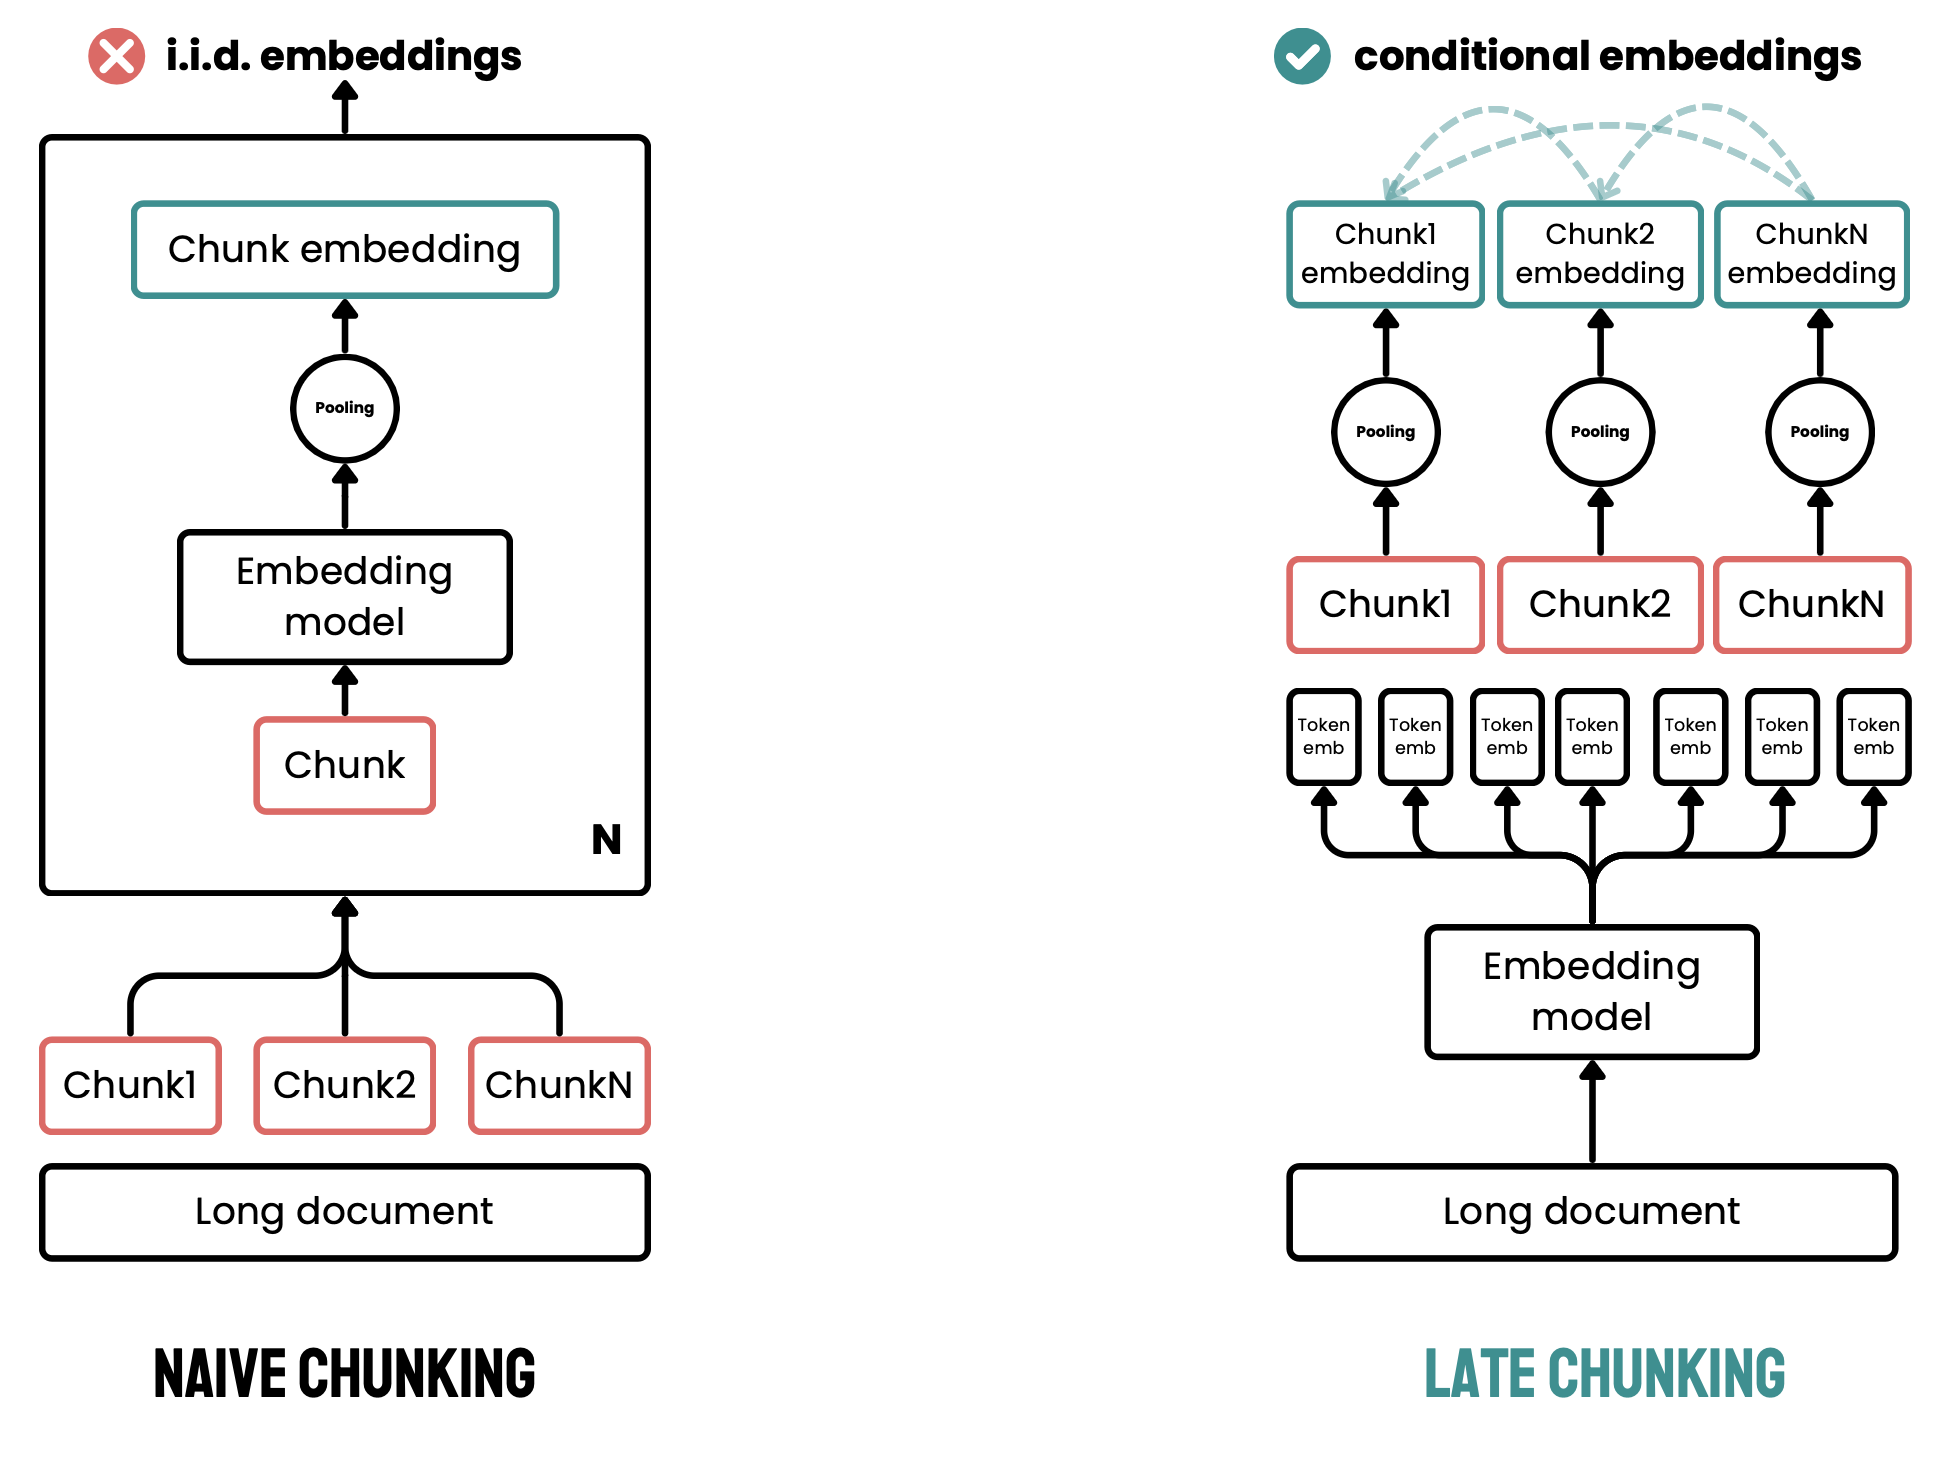
\includegraphics[width=\textwidth]{images/chapter3/late_chunking.png}
    \caption{Visualization of the Late Chunking algorithm (right) compared to naive chunking (left). Image from Günther et al. (2025) \autocite{günther2025latechunkingcontextualchunk}.}
    \label{fig:late_chunking}
\end{figure}

\begin{algorithm}
\caption{Late Chunking}
\label{alg:late_chunking}
\begin{algorithmic}[1]
\Procedure{LateChunking}{document, chunk\_boundaries}
    \State $tokens \gets \text{tokenize}(document)$
    \State $\omega_1, \dots, \omega_m \gets \text{Transformer}(tokens)$ \Comment{Generate token-level embeddings}
    \State $token\_spans \gets \text{get\_token\_spans}(document, tokens)$
    \State $chunk\_token\_indices \gets []$
    \For{each $chunk$ in $chunk\_boundaries$}
        \State $start\_char, end\_char \gets chunk$
        \State $start\_token \gets \text{find\_token\_at\_char}(token\_spans, start\_char)$
        \State $end\_token \gets \text{find\_token\_at\_char}(token\_spans, end\_char)$
        \State append $(start\_token, end\_token)$ to $chunk\_token\_indices$
    \EndFor
    \State $chunk\_embeddings \gets []$
    \For{each $start\_idx, end\_idx$ in $chunk\_token\_indices$}
        \State $token\_vectors\_for\_chunk \gets \omega_{start\_idx}, \dots, \omega_{end\_idx}$
        \State $embedding \gets \text{MeanPool}(token\_vectors\_for\_chunk)$
        \State append $embedding$ to $chunk\_embeddings$
    \EndFor
    \State \Return $chunk\_embeddings$
\EndProcedure
\end{algorithmic}
\end{algorithm}